\newlength\bottomstripheight%
\setlength{\bottomstripheight}{.25\textheight}%
%
\begin{minipage}[t]{\textwidth}%
\vskip0pt%
\textcolor{BaseColor}{%
\rule{\textwidth}{.2mm}%
}\hfill%
%
%
\begin{minipage}[b][\bottomstripheight][b]{.48\textwidth}%
%
\cblock{BaseColor}{}{Training Results}{}%
\small%
We first initialize a feed-forward architecture using a small percentage of its parameters. We then respectively train the net with standard SGD, sparsity enforcing ProxGD and \emph{LinBreg}.
\begin{figure}
\begin{minipage}{.7\textwidth}%
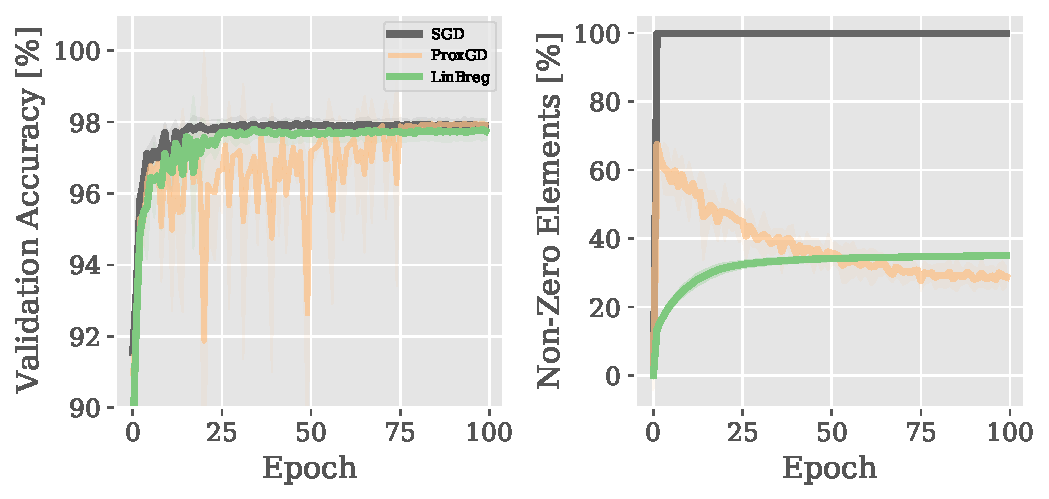
\includegraphics[width=\textwidth, trim= 0cm 0cm 0cm 0cm,clip]{atelier/SGDvsBreg_small.pdf}
\end{minipage}%
\begin{minipage}{.3\textwidth}%
\caption{\small Comparison of vanilla SGD, \LinBreg{}, and ProxGD.
The curves show the averaged train accuracies sparsity.}
\end{minipage}%
\end{figure}%
%
%
%
Additionally, we compare ourselves to a variant of the LASSO \cite{??} regularizer on the CIFAR10 \cite{Krizhevsky09} dataset, employing a ResNet-18 \cite{he2015delving}.
%
%
%
\begin{table}[htb]
\scriptsize
\begin{minipage}{.69\textwidth}%
\begin{tabularx}{\textwidth}{|c||c c|R R|}
Strategy & Optimizer & 
$\mathrm{N}_{\mathrm{total}}$ in [\%] & 
Test Acc&Train Acc\\
\hhline{|=====|}
\multirow{2}{*}{Vanilla}
&SGD with momentum &100.0&92.15&99.8\%\\
&Adam &100.0&93.6&100.0\%\\
\hhline{-----}
\multirow{2}{*}{Lasso}
        &Adam &99.7&91.1 &100\\
        &Adam + thresh.&3.0&90.0 &99.8\\
\hhline{-----}
\multirow{2}{*}{\bf{\small Bregman}}
                &\LinBreg{} &5.5&90.9&99.5\\
                &\LinBreg{} + thresh.&3.4&90.2&99.4\\
\end{tabularx}
\end{minipage}%
\begin{minipage}{.01\textwidth}%
\phantom{2}
\end{minipage}%
%
\begin{minipage}{.3\textwidth}%
\caption{Sparsity levels and accuracies on the CIFAR-10 data set.}\label{tab:CIFAR}
\end{minipage}
\end{table}
%
%
%
%
%
%
\vfill%
\vphantom{.}
\end{minipage}%
%
\hfill%
%
\tbox{%
\noindent\begin{minipage}[b][\bottomstripheight][b]{.005\textwidth}%
%
\begin{center}
\textcolor{BaseColor}{%
\rule{.2mm}{\bottomstripheight}%
}
\end{center}
\end{minipage}%
}%
%
\hfill%
%
%
%
%
%
%
%
\noindent\begin{minipage}[b][\bottomstripheight][b]{.48\textwidth}%
%
\cblock{BaseColor}{}{NAS with Bregman}{}%
\small%
We initialize a sparse multi-layer perceptron with the same amount of active neurons in each layer. Training this net in order to perform a denoising task reveals an autoencoder architecture. 

\begin{figure}%
\begin{minipage}{.3\textwidth}%
\caption{Architecture design for denoising: \LinBreg{} unveils an autoencoder.}
\end{minipage}%
\begin{minipage}{.7\textwidth}%
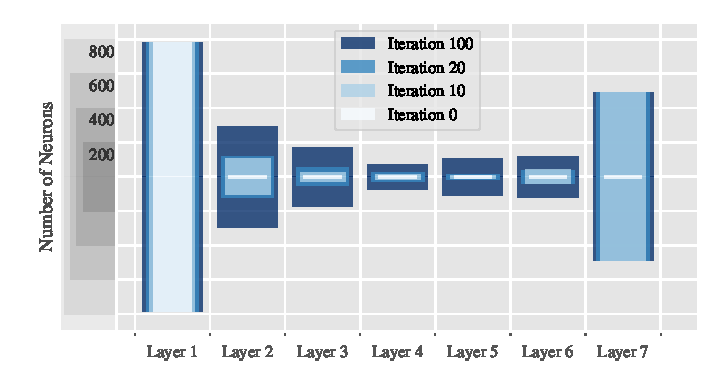
\includegraphics[width=\textwidth]{atelier/Encoder_3.pdf}
\end{minipage}%
\end{figure}
%
%
%
\cblock{BaseColor}{BaseColorD}{\normalsize References}{%
\AtNextBibliography{\footnotesize}
\printbibliography[heading=none]
}


\vfill%
\vphantom{.}
\end{minipage}%
\end{minipage}%
%

